\chapter{Project Goals and Requirements}
\label{ch:goals}

The primary objective of the ft\_transcendence project is to create a comprehensive and engaging web-based Pong game experience. This involves not only replicating the core gameplay but also integrating modern web technologies, robust security features, and advanced functionalities. The specific goals defined for this project are as follows:

\begin{itemize}
    \item \textbf{Deliver a Single-Page Application (SPA):} The game must be playable directly in the browser without requiring page reloads, offering a seamless user experience.
    
    \item \textbf{Provide Secure User Management:} Implement a secure system for user registration, login, and profile management. This includes:
    \begin{itemize}
        \item Native credential authentication (username/password).
        \item Integration with the 42 Intra OAuth 2.0 provider.
        \item Secure session management using JSON Web Tokens (JWT) stored in cookies.
        \item Optional Time-based One-Time Password (TOTP) Two-Factor Authentication (2FA) for enhanced security.
    \end{itemize}
    
    \item \textbf{Offer Multiple Game Modes:} Cater to different player preferences by providing several ways to play Pong:
    \begin{itemize}
        \item 1 vs 1 online matches against other registered users.
        \item 1 vs AI matches against a computer-controlled opponent.
        \item Local 4-player multiplayer on a single screen.
        \item Structured tournaments with bracket progression.
    \end{itemize}
    
    \item \textbf{Persist Data Securely and Reliably:} Store user data, match history, and tournament results using appropriate technologies:
    \begin{itemize}
        \item Utilize a \textbf{PostgreSQL} relational database for general application data, user profiles, and individual match results.
        \item Record final tournament results immutably on an \textbf{Ethereum sidechain} (using a Proof-of-Authority consensus mechanism) to ensure data integrity and verifiability.
    \end{itemize}
    
    \item \textbf{Expose a Clean RESTful API:} Develop a well-documented Application Programming Interface (API) using Django Rest Framework (DRF). This allows the frontend SPA to communicate with the backend and enables potential future development of alternative clients (e.g., command-line tools, mobile applications).
    
    \item \textbf{Implement Production-Grade DevOps Practices:} Ensure the application is easy to deploy, manage, and monitor using industry-standard tools and practices:
    \begin{itemize}
        \item Containerize all application components (frontend, backend, database, etc.) using \textbf{Docker}.
        \item Orchestrate the multi-container application stack using \textbf{Docker-Compose} for easy setup and deployment.
        \item Utilize \textbf{Nginx} as a reverse proxy to handle incoming traffic, serve static frontend assets, and manage HTTPS termination.
        \item Integrate centralized logging and monitoring using the \textbf{ELK stack} (Elasticsearch, Kibana) to provide insights into application performance and potential issues.
        \item Provide convenient management commands using a \textbf{Makefile}.
    \end{itemize}
\end{itemize}

These goals collectively aim to produce a polished, secure, and feature-rich web application that showcases proficiency in full-stack development, DevOps, and blockchain integration within the context of a familiar and engaging game.

\chapter{Software Development Life Cycle (SDLC)}
\label{ch:sdlc}

This chapter outlines our approach to developing the project following the Software Development Life Cycle (SDLC) methodology. We cover the key phases including requirement analysis, design, implementation, testing, and evolution (maintenance). Each phase builds upon the previous one, ensuring a systematic and comprehensive development process.

The Software Development Life Cycle (SDLC) for this project follows a modified Waterfall model, incorporating Agile elements to enhance flexibility and iterative improvements. While the Waterfall approach provided a structured framework for sequential stages like requirement analysis, design, implementation, and testing, we introduced Agile practices such as ongoing feedback and peer-reviewed GitHub pull requests (PRs). This process of PR reviews allowed team members to give feedback on each other's code, identify potential issues early, and ensure quality and consistency across different modules. By integrating peer-reviewed PRs, we facilitated continuous testing, collaborative refinement, and adherence to best practices throughout the development. This hybrid methodology helped us achieve a balance of systematic progression with opportunities for iteration and improvement based on team insights.

\section{Requirement Analysis}

Requirement Analysis is the first and one of the most crucial phases of the Software Development Life Cycle (SDLC). During this phase, the focus is on gathering detailed requirements and defining the project’s objectives. This phase helps ensure that the project starts on the right track, with a clear understanding of what needs to be built, why it is being built, and how it will be used. Proper requirement analysis sets the foundation for all subsequent stages of the software development process.
By understanding and addressing potential risks early, such as technical feasibility, resource constraints, or user expectations, the project can avoid delays or even a potential failure. Additionally,  proper documentation and agreement on requirements ensure that all members are on the same page, reducing miscommunication and conflicts later. 
Starting with a solid foundation minimizes misunderstandings and scope changes and sets the stage for successful project execution. In order to properly gather the requirements, it was necessary to choose which modules best fit the team skills and interests. Initially some modules were set, and others were flagged as “interested”, that the team would do according to the project development. 


\section{Modules Implemented}

After a careful analysis, the following core modules and features were implemented, aligning with the project goals:

\begin{enumerate}
    \item \textbf{Backend Framework:} Utilized Django (Python framework) to build a robust and scalable backend, providing RESTful APIs via Django Rest Framework (DRF).
    \item \textbf{Frontend Implementation:} Developed a Single-Page Application (SPA) using Vanilla JavaScript (ES6+) for interactivity and HTML5 Canvas for game rendering. Leveraged Bootstrap 5 as a toolkit for responsive design and UI components.
    \item \textbf{Database Integration:} Employed PostgreSQL as the primary relational database for storing user data, match history, and application settings, integrated via the Django ORM.
    \item \textbf{User Management and Authentication:} Implemented comprehensive user management features including secure registration, profiles (with avatars and stats), and friend lists. Supported multiple authentication methods: native credentials, 42 Intra OAuth 2.0.
    \item \textbf{Enhanced Security:} Integrated JWT (JSON Web Tokens) via \texttt{djangorestframework-simplejwt} for stateless session management (using secure HttpOnly cookies) and provided optional TOTP-based Two-Factor Authentication (2FA) using \texttt{django-otp}.
    \item \textbf{Core Gameplay (Pong):} Developed the classic Pong game with various modes:
        \begin{itemize}
            \item 1 vs 1 online matches.
            \item 1 vs AI opponent.
            \item Local multiplayer (up to 4 players).
            \item Structured tournaments with bracket display.
        \end{itemize}
    \item \textbf{Blockchain for Tournaments:} Integrated an Ethereum sidechain (Proof-of-Authority) to immutably record tournament results using Solidity smart contracts and Web3.py interaction from the backend.
    \item \textbf{Game Customization:} Provided options for users to customize certain aspects of their game experience (details may vary, e.g., potentially paddle appearance or simple settings).
    \item \textbf{DevOps and Containerization:} Utilized Docker and Docker Compose to containerize all services (backend, frontend, database, Nginx, ELK, Geth) for consistent deployment and orchestration.
    \item \textbf{Monitoring:} Integrated the ELK stack (Elasticsearch, Kibana) for centralized logging and application monitoring.
    \item \textbf{Accessibility Considerations:} Included features to enhance accessibility, such as support for keyboard navigation and considerations for visually impaired users (e.g., high-contrast options).
\end{enumerate}

\section{Design the System Architecture}
The Design Phase is the second major stage in the SDLC, where the focus transitions from defining system requirements to designing how the system will meet those requirements. The project architecture is divided into independent services, each running in Docker containers, to enhance scalability and maintainability.

For the database, \texttt{PostgreSQL} is selected to ensure data integrity and seamless integration with \texttt{Django}, while \texttt{Bootstrap} is utilized for creating a responsive and accessible UI design on the frontend.

In terms of security design, secure login methods, including 42 login or username, with Two-Factor Authentication (2FA) and JSON Web Tokens (JWT) for authentication, are implemented.

During this stage, the initial draft of the website workflow and the structure of page linkages were established in a group meeting. This draft outlined user navigation through the site, detailing the connections between different pages to ensure a coherent user experience. This early planning phase was crucial for aligning development efforts across various teams, such as frontend design, backend functionality, and game integration, setting the foundation for subsequent implementation stages.

\begin{figure}[H]
    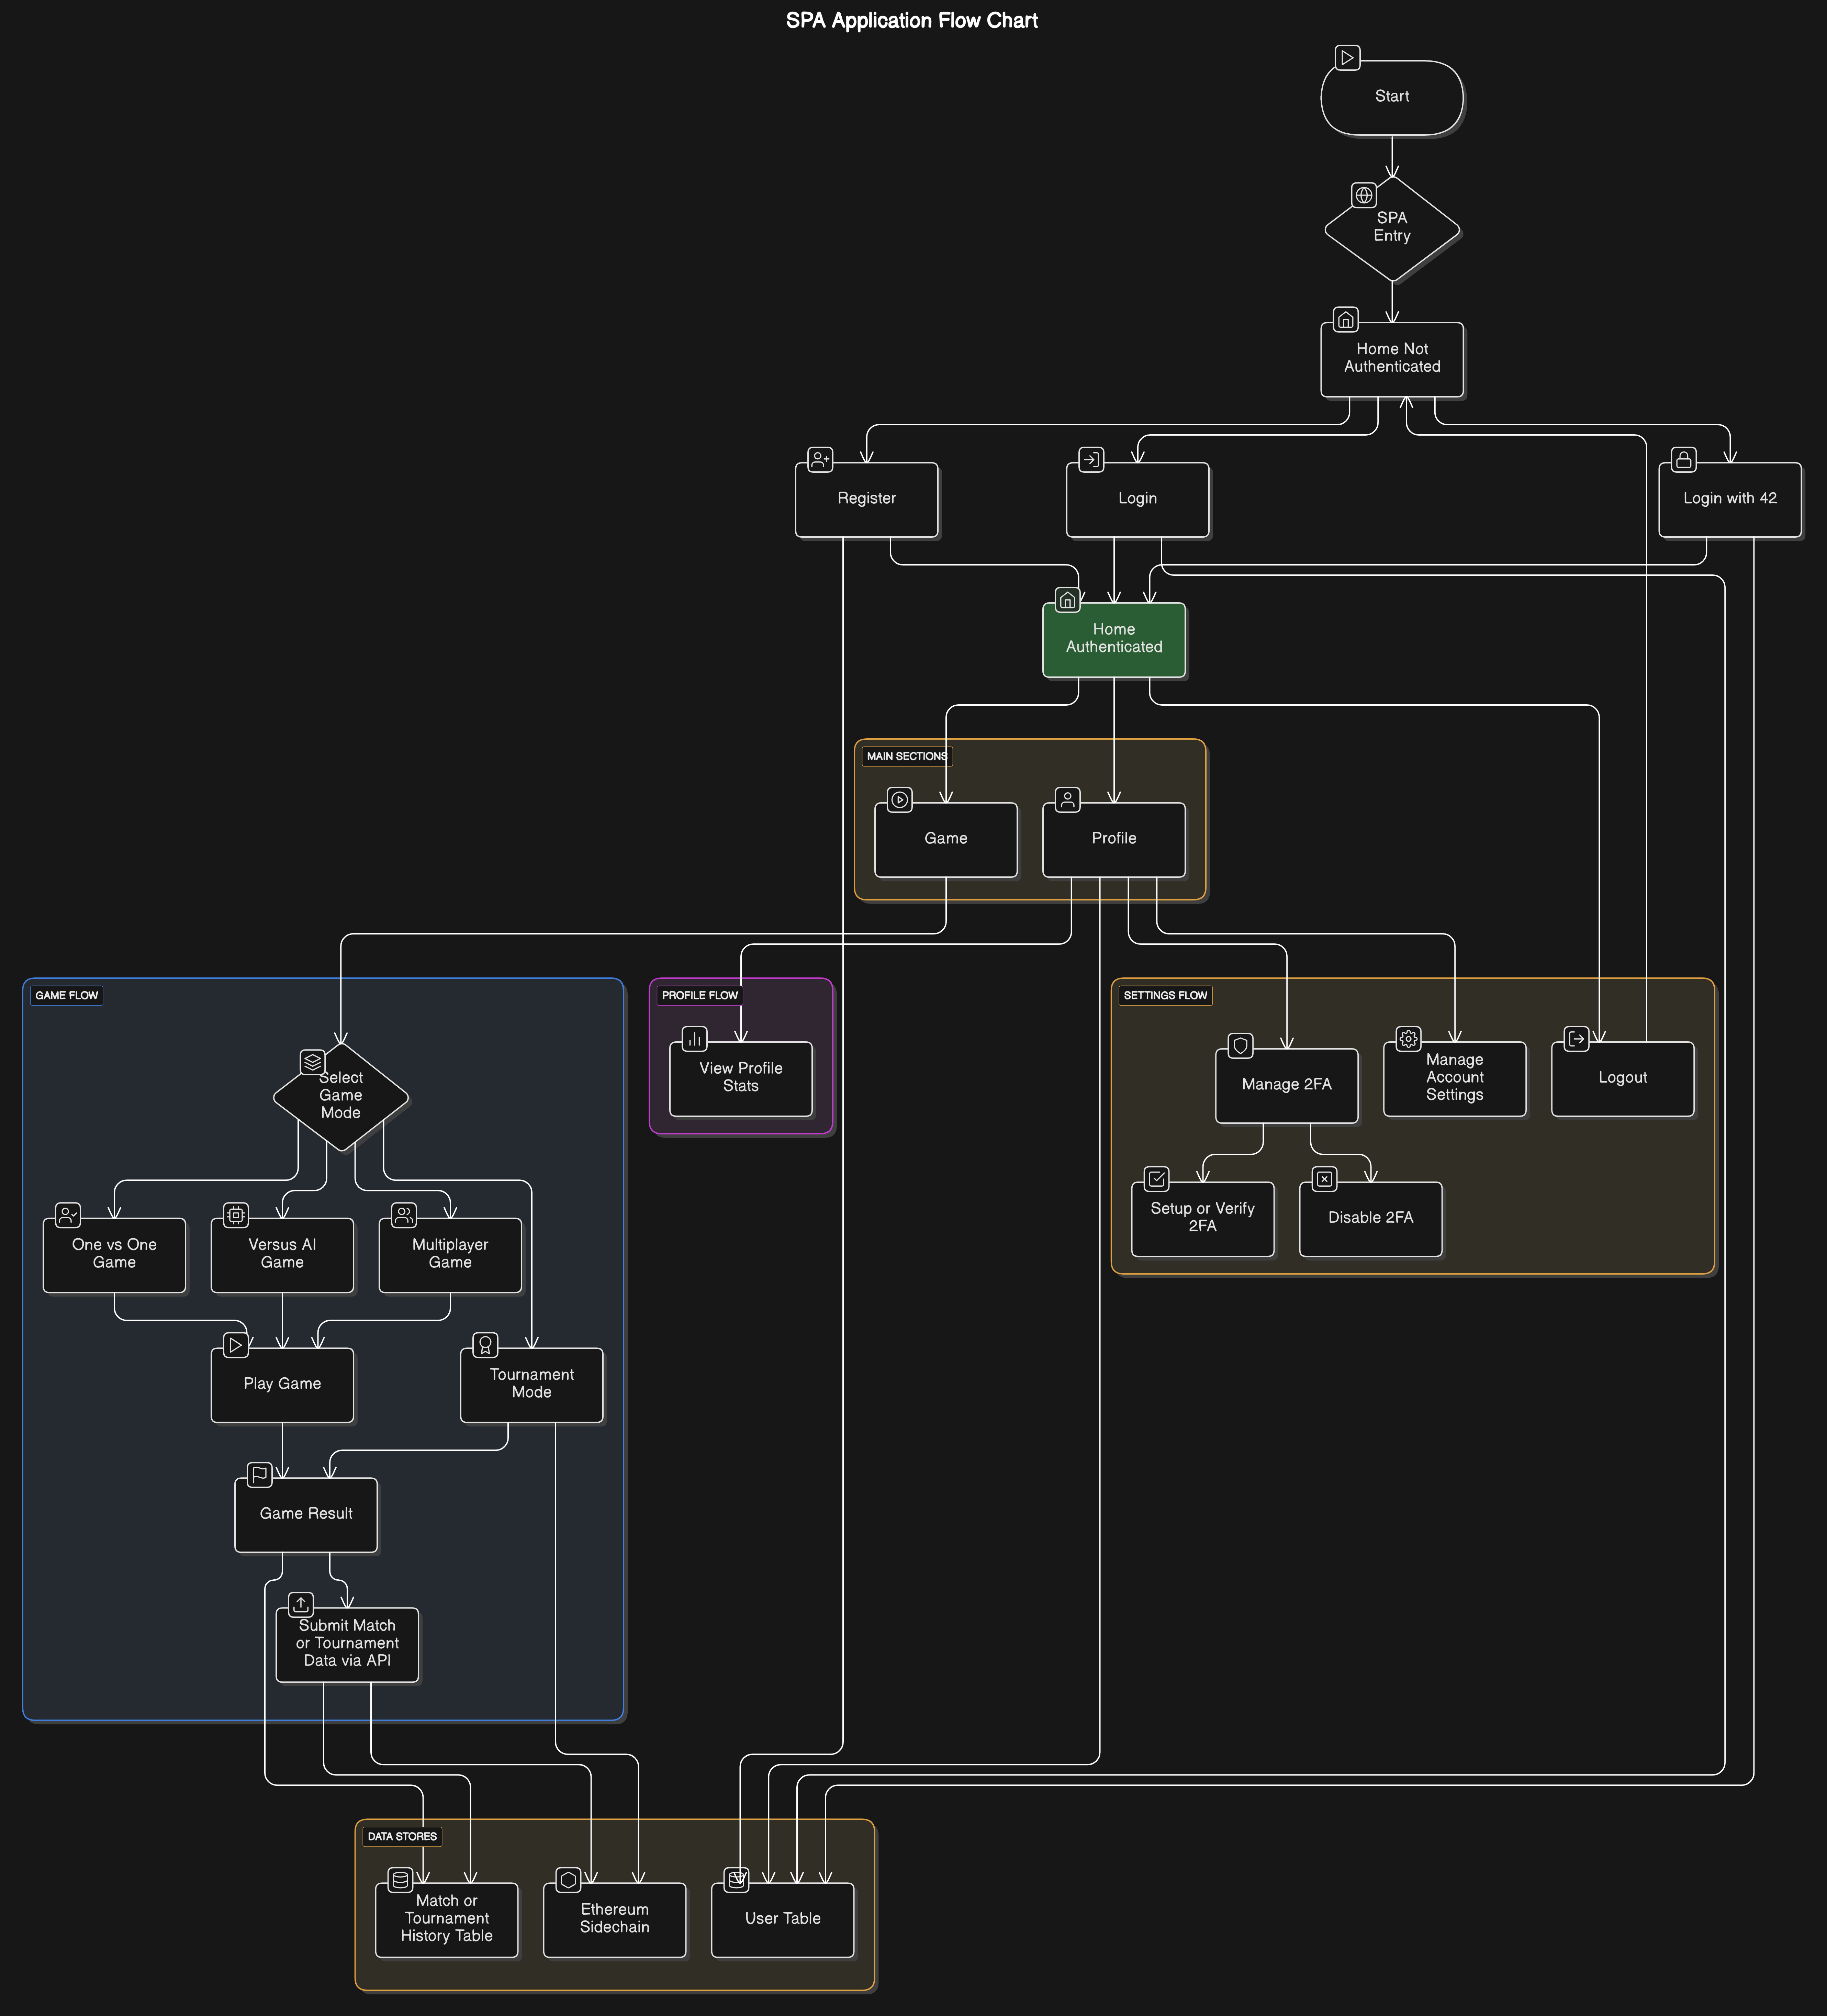
\includegraphics[width=1\linewidth]{Figures/images/workflow.png}
    \caption{Workflow}
    \label{fig:workflow}
\end{figure}


\section{Implementation}
The implementation step involves developing the actual code and functionality based on the design specifications. For this web application project, the implementation step was broken down into the following main aspects:
\begin{itemize}
    \item \textbf{Backend Development:} We developed the core functionality using Django, ensuring the backend supported all game features and incorporated robust security protocols. The backend manages user data securely, supports multiple game modes, and provides RESTful APIs for frontend interaction. The application is safeguarded against SQL injection and Cross-Site Scripting (XSS) attacks through Django's inherent security features. Specifically, Django mitigates SQL injection risks by automatically escaping user inputs and providing secure query methods. The framework's ORM functions such as \texttt{.filter()}, \texttt{.get()}, and \texttt{.exclude()} incorporate mechanisms that prevent execution of malicious SQL code. Additionally, we implemented non-root user execution in our Docker containers to address privilege escalation vulnerabilities.
    
    \item \textbf{Frontend Development:} We built a responsive user interface using Bootstrap 5, incorporating accessibility features such as high-contrast themes and keyboard navigation using the "tab" key. The frontend adapts seamlessly across different devices and screen sizes, offering an inclusive experience for users, including those with visual impairments. We implemented the SPA architecture using Vanilla JavaScript to minimize dependencies while maintaining performance.
    
    \item \textbf{Game Development:} We implemented the core Pong game mechanics with customization options for different skill levels and settings. This included developing interactive controls, configuring adjustable game parameters, and ensuring real-time responsiveness through optimized Canvas rendering. The game includes comprehensive user history tracking to record and display individual gameplay statistics.
    
    \item \textbf{User History and Matchmaking:} We integrated a user history tracking system to securely store game outcomes in PostgreSQL and ensure data is always up to date. These additions enhance user engagement by providing detailed gameplay statistics and facilitating seamless matchmaking for competitive play.
    
    \item \textbf{User Management and Authentication:} We implemented secure user management features with both native credentials and 42 OAuth authentication options, plus optional TOTP-based Two-Factor Authentication. Users can select unique display names, update their information, and upload avatars. Additional features include managing friend lists, viewing online status, and accessing user profiles with comprehensive statistics. All user management functionalities comply with best practices for secure authentication using JWT stored in HttpOnly cookies.
    
    \item \textbf{Development Workflow:} To enable simultaneous work across different components, we implemented a branching strategy on GitHub where each task had its dedicated branch. This approach allowed team members to work independently while preserving the integrity of the main branch. Before merging changes, a peer review process ensured code quality and caught potential issues early. Figure \ref{fig:workflow} illustrates this workflow from our development period (February to April 2025), demonstrating how multiple branches facilitated collaborative development and quality assurance.
\end{itemize}

\section{Testing the application and its functionalities}

Testing phase in the SDLC ensures that the web application is functional, secure, user-friendly, and meets all requirements. Focusing on Pong game web application, testing can be broken down into several types, each targeting different aspects of the system:
\begin{itemize}
    \item \textbf{Unit Testing:} Test individual components of the application in isolation to ensure their functionality is correct. Examples include verifying user authentication mechanisms, game logic (such as ball physics and paddle movements in Pong), and database interactions. These tests validate core functionality like game rules, user input handling, and match outcome determination.
    
    \item \textbf{Integration Testing:} After unit testing, it is necessary to test the interactions between multiple components. Integration testing includes verifying the communication between the frontend and backend (e.g., submitting a login request and receiving the correct response, game management, authentication, user profiles), and ensuring data is correctly stored, retrieved, updated, and deleted from the PostgreSQL database. It was also necessary to perform tests to confirm that the user history and matchmaking system of the game were operating seamlessly, and data flows correctly across services.
    
    \item \textbf{Functional Testing:} The main goal is to verify that the application meets all functional requirements and works as intended. This is done by testing the game functionality (e.g., in the Pong game, issues like ball collision detection, paddle movement, multiplayer synchronization, adjusting ball and paddle speed, difficulty levels, and sound settings should be analyzed). For authentication and security, it is necessary to check if both login methods (42 login and username), 2FA setup, and JWT session management are properly working, as well as if a non-logged user can access the content restricted to a logged user. In addition, the logout option was also tested to ensure that the session was properly finished. Lastly, user management features like user registration, profile updates, password resets, and tournament participation were analyzed.
    
    \item \textbf{Usability Testing:} This next step evaluates the application's user interface and experience, ensuring it is intuitive and accessible for users. The main tests were focused on testing the web application on different devices (desktop, tablet, mobile) to ensure the UI is responsive and easy to use, and checking that all accessibility features (e.g., high-contrast colors, keyboard navigation) work correctly and comply with accessibility standards. After that, the focus shifted to gathering feedback from users on the game's interface, navigation, and overall experience to identify potential improvements.
    
    \item \textbf{Compatibility Testing:} The goal is to ensure the application functions consistently across different environments. For this application, the browsers “Chrome” (last available version) and “Firefox” were chosen, and in this sense, all tests were performed on both browsers.
\end{itemize}

In addition to the tests mentioned above, CI/CD was integrated as an automation tool within the GitHub (Figure 2) workflow to prevent commits that would fail the build. This approach proved highly effective, minimizing rework and ensuring that each merge met the minimum standards required for committing to the main branch.


% \section{Testing the application}
% We periodically tested the code after each stage of code implementation to ensure that the code was running properly before moving on to the next stage. This involved a variety of tests, including unit testing to validate individual components, integration tests to assess how different parts of the system worked together, and user tests to gather feedback from real users. This testing strategy allowed us to identify and resolve bugs early, ensuring a smoother development process as we built the code.

% \section{Future improvements}
% After deployment, we need to focus on system maintenance and consider how we can update the game. This includes monitoring performance, addressing any issues that arise, and implementing enhancements based on user feedback. We should also plan for regular updates to introduce new features, fix bugs, and ensure the game remains engaging and enjoyable for players.
